%\documentclass[a4paper]{article}
\documentclass[usenatbib]{mn2e}
%% Language and font encodings
\usepackage[english]{babel}
\usepackage[utf8x]{inputenc}
\usepackage[T1]{fontenc}

\usepackage{natbib}
%% Sets page size and margins
\usepackage[a4paper,top=3cm,bottom=2cm,left=3cm,right=3cm,marginparwidth=1.75cm]{geometry}

%% Useful packages
\usepackage{amsmath}
\usepackage{graphicx}
\usepackage[colorinlistoftodos]{todonotes}
\usepackage[colorlinks=true, allcolors=blue]{hyperref}

\newcommand       \apj  {ApJ}
\newcommand       \apjl  {ApJL}
\newcommand       \apjs  {ApJS}
\newcommand       \aj  {AJ}
\newcommand       \aap {A \& Ap.}
\newcommand       \mnras {MNRAS}
\newcommand       \nat {Nature}
\newcommand       \araa {ARA\&A}
\newcommand       \physrep {Phys.~Reports}
\newcommand       \prd {PhysRevD}

\title{Photo-z for LSST: comparison of PDFs}
\author{LSST PZ WG}

\begin{document}
\maketitle

\begin{abstract}
The rationale: - to test different PZ codes on DC1 simulations 

- to focus on the pdf p(z) and to compare results via various metrics

- This is a good way to compare quantitatively results by various groups, and also to credit collaborators, 
\end{abstract}

The timeline for the paper:

Which Journal? AJ, ApJ, MNRAS? (leaning toward MNRAS, no page charge…) 

\section{Introduction}

(Sam Schmidt, Ofer Lahav, Jeff Newman, Alex Malz)

%* The challenges of PZ in LSST 
%* Many papers compared point estimates; here we focus on the pdf $p(z)$
We are entering a new regime with Stage III and Stage IV dark energy experiments[add text about DES, LSST, WFIRST, Euclid, along with references].  The move to imaging based surveys, rather than spectroscopic based, for cosmological measurements makes proper understanding of photometric redshifts ("photo-z's") of paramount importance, as all cosmological distance measures for statistical samples will be dependent on photo-z measurements.  As we push to fainter magnitudes and deeper imaging, we expand our samples to include lower luminosity and higher redshift galaxies.  These populations introduce major degeneracies, for example the Lyman break/Balmer break degeneracy, that were not present in previous large area surveys (SDSS, 2MASS, etc...[spell out and put references]).  The increased sample size that comes with the added depth means that stringent constraints on photo-z accuracy are necessary if systematic errors are not to dominate the statistical errors.  The LSST Science Requirements Document (SRD)\footnote{available at:https://docushare.lsstcorp.org/docushare/dsweb/Get/LPM-17} lists the photometric redshift goals for a magnitude limited sample with $i<25$ as: root mean square error of $\sigma<0.02(1+z)$; $3\sigma$ "catastrophic outlier'' rate below 10\%; bias below 0.003.  Note that at the time the SRD was written, these goals were stated in terms of one signle number estimate of photometric redshift for each galaxy.  Many of the previous studies of photo-z performance focused on single point estimates of the redshift.  Such a simple redshift measure fails to capture the full information in the presence redshift degeneracies, where multiple redshift solutions have considerable likelihood.  In this paper we focus on the full probability density function (PDF), or p(z) for each galaxy.  [What else to say about p(z)?]

In order to meet these ambitious goals for photo-z accuracy, every aspect of photo-z estimation will have to be optimized: the algorithms employed, both template and machine-learning based (both in design and implementation),  the spectroscopic data used as a training set for machine learning algorithms or to estimate template sets and train Bayesian priors in template based methods
storage formats for p(z) that are accurate enough for all science cases while simultaneously compact enough to fit in a reasonably spec'd database.
In this paper, we focus on current generation photo-z algorithms, comparing the performance of several of the most widely employed codes.  This is similar in spirit to the PHoto-z Accuracy And Testing \citep[PHAT,][]{Hildebrandt:10} effort, though that comparison used many more photometric bands, and compared only point-estimates.  The Dark Energy Survey (DES, REFERENCE!) compared several codes, both for point estimates \citep[]{Sanchez:14}, and using sum of p(z) for collections of galaxies in tomographic bins \citep[]{Bonnett:16}.
(mention that this is not the correct way to combine and cite Malz in prep).  

ToDo: Mention SRM, multiple data challenges (DCs), and that this is the first of multiple papers, which will grow in sophistication.

In order to isolate the effects of the codes from issues with the training set and template library, we will use two sets of simulated galaxies and construct a training sample that is {\it representative and spanning}.  We will address the very important issue of incomplete spectroscopic coverage in a future paper.

The outline of the paper is as follows: in \S\,\ref{pzcodes} we describe the current generation codes employed in the paper; in \S\,\ref{sims} we present the two simulated data sets; in \S\,\ref{metrics} we discuss the "meaning'' of redshift PDFs, and lay out the metrics that we use to evaluate them; in \S\,\ref{results} we show our results and compare the performance of the codes; in \S\,\ref{discussion} we offer our conclusions and discuss future extensions of this work.

\section{PZ Codes}\label{pzcodes}

(Sam Schmidt, Rongpu Zhou, Ibrahim Almosallam, Eric Nuss, Johann Cohen Tanugi, John Soo, Alex Malz)

* Existing training and testing codes (briefly, possibly a Table)

* What is the meaning of $p(z)$ in different codes? (Ofer) 

* ACTION ITEM: who has what code in place? Are any important codes missing?

* Action item: make a table of codes (Sam)

\subsection{BPZ}\label{sec:BPZ}
\texttt{BPZ}\footnote{We use \texttt{BPZ v 1.99.3}, available at: \url{http://www.stsci.edu/~dcoe/BPZ/}} \citep[Bayesian Photometric-$z$, see][for details]{Benitez:00} is a template-based photo-$z$ code which compares the expected colors (C) calculated for a set of SED types/templates (T) to the actual observed colors to calculate the likelihood of observing colors $p(C|z,T)$ at each redshift for each type.  The code employs an empirically determined Bayesian prior in apparent magnitude ($m_0$) and SED-type.  Assuming that the SED-types are spanning and exclusive, we can determine the redshift posterior by marginalizing over all SED-types with a simple sum (Eq.~3 from \citet[]{Benitez:00}):
\begin{equation}
p(z|C,m_0)\,\propto\, \sum_{T}p(z,T|m_0)\,p(C|z,T)
\end{equation}
\noindent where the first term is the Bayesian prior and the second term is the traditional likelihood.  The prior is assumed to have the form: $p(z,T|m_0) = p(T|m_0)\,p(z|T,m_0)$that is, it parameterizes the prior as an evolving type fraction with apparent magnitude, combined with a prior on the expected redshift probability distribution as a function of both apparent magnitude and SED-type.\\

The template set used for the Buzzard dataset is the set of 100 SEDs described in Section~\ref{sec:buzztemplates}, and use the 129 Brown SEDs for the Galacticus dataset.  For both datasets, to keep the number of free parameters to a manageable level, the SEDs in the training set are sorted by rest-frame $u-g$ colour and split into three ``broad'' SED classes, equivalent to the \texttt{E}, \texttt{Sp} and \texttt{Im/SB} types in \citet[]{Benitez:00}.  We assume the same functional form for the Bayesian prios as used by \citet[]{Benitez:00}, and utilize the training-set galaxies with known SED-type, redshift, and apparent magnitude to determine the type fractions and the best fit for the 11 free parameters of the prior.  For photo-$z$ point estimate we use the \texttt{Z\_B} output parameter.  For the type-marginalized p(z) is generated by setting the parameter \texttt{PROBS\_LITE=TRUE}.

\subsection{ANNz2}\label{sec:annz2}
ANNz2\footnote{\url{https://github.com/IftachSadeh/ANNZ}} \citep{sadeh_annz2:_2016} is a machine learning photo-z estimation method which uses the Toolkit for Multivariate Data Analysis (TMVA) with ROOT\footnote{\url{http://tmva.sourceforge.net/}}. It is a powerful package that incorporates several machine learning algorithms including ANN, boosted decision tree (BDT) and k-nearest neighbour (KNN). ANNz2 can run multiple machine learning algorithms for a single training and outputs photo-z's based on a weighted average of their performances.

Other than the usual regression method to obtain point estimates for photo-z's, ANNz2 is also able to produce redshift posterior probability distributions $P(z)$, conduct classification and support reweighting between samples. The pdfs are produced by propagating the intrinsic uncertainty on the input parameters and the uncertainty in the machine learning method to the expected photo-z solution. ANNz2 also differs from many other codes by its presentation of photo-z uncertainty, it derives uncertainties using the KNN method: first it estimates the photo-z bias between each object and a fixed number of nearest neighbours in parameter space, it then takes the 68th percentile width of the distribution of the bias. This asserts that objects with similar photometric properties should have similar uncertainties, and this error presentation has been shown to perform better than the former \citep{sadeh_annz2:_2016}.

ANNz2 produces four point estimates for each run, but in this study we use the pdf average photo-z, which is the mean photo-z calculated over the pdf. The pdf average photo-z will act as the best point estimate photo-z output for ANNz2. In this study, a set of 5 ANNs with different random seeds are used during each training. 

\section{The DC1 simulations}\label{sims}

(Sam Schmidt, Eve Kovacs, Tina Peters)

* Describe the simulations (Sam, Eve, etc…)

* Describe the template sets (Sam)

* Discuss limitations wrt to the galaxies in nature (Eve, Tina Peters)

In order to test the current generation codes, we created two simulated datasets.  The simulations are completely catalog-based, with no image construction or mock measurements made [phrase this better].  We describe these in detail below.  

\subsection{Buzzard (what should we call this officially?)}\label{buzzard}

   The Buzzard-highres-v1.0 catalog construction began with an dark matter only simulation.  This N-body simulation contained 2048$^3$ particles in a 400 Mpc/h box.  [HOW MANY SNAPSHOTS?] time snapshots were saved in order to construct a lightcone [Any smoothing/interpolation done between snapshots?].  Dark matter halos were identified using the {\it Rockstar} software package \citep[]{Behroozi:13}.  These dark matter halos were populated with galaxies with a stellar mass and  absolute r-band magnitude (in the [SDSS or DES?] system) determined using a sub-halo abundance matching model constrained to match both projected two-point galaxy clustering statistics and an observed conditional stellar mass function \citep[]{Reddick:13}. 

To assign an spectral energy distribution (SED) to each galaxy, the Adding Density Dependent Spectral Energy Distributions (ADDSEDS) [Is there a reference paper for ADDSEDS?] procedure was used.  This consisted of training an empirical relation between absolute r-band magnitude, local galaxy density, and SED using a sample of $\sim 5e^{5}$ galaxies from the Sloan Digital Sky Survey [PUT PROPER REF FOR specz sample]. [should we mention that we actually only have 5 NNMF components? and they are same as k-correct?].  The distance to the projected fifth-nearest neighbor was used as a proxy for local density in the SDSS training sample.  For each simulated galaxy, a ``random'' [How exactly is this done? random in a certain volume of parameter space, maybe?] galaxy with ``similar'' [again, this needs detail] absolute r-band magnitude and local galaxy density was chosen from the training set, and that training galaxy's SED was assigned to the simulated galaxy.  Given the SED, absolute r-band magnitude, and redshift, we computed apparent magnitudes in the six LSST filter passbands, $ugrizy$.  We assigned magnitude errors in the six bands using the simple model described in Section 3.2 of \citet[]{Ivezic:08}, assuming full 10-year depth observations had been completed [should we list the number of visits and such?].

The total catalog covered 400 square degrees and contained 238 million galaxies to an apparent magnitude limit of $r\!=\!29$ and spanning the redshift range $0\!<\!z\!\leq\!8.7$.  This catalog contained two orders of magnitude more galaxies than were needed for this study, so only $\sim\!8$ square degrees were used.  Systematic problems with galaxy colours above $z\!>\!2$ were observed, so the catalog was trimmed to include only galaxies in the redshift range$0\!<\!z\!\leq\!2.0$.  A random subset of the the remaining galaxies was chose, and placed, again at random, into either a "training'' set (10\% of the sample), for which the galaxies true redshifts will be supplied, or a "test'' set (the remaining 90\% of the sample), for which each code will need to predict a redshift PDF for each galaxy. The resulting catalogues contain 111,171 training galaxies and 1,000,883 test galaxies.

\subsubsection{Templates}\label{sec:buzztemplates}
[Describe the templates here? Or describe them earlier?]

\subsection{Galacticus [ABC?]}\label{Galacticus}

\section{Metrics for quantifying pdf comparisons}\label{metrics}

(Alex Malz, Rongpu Zhou, Jeff Newman, Ofer Lahav)

What is the meaning of “pdf”? 

The overloaded "$p(z)$" is a widespread abuse of notation; we would like the outputs of our codes to be interpretable as probabilities.  Each PDF is a posterior probability distribution conditioned on a number of things that will differ depending on the method used to derive it; these things will certainly include the photometry associated with the galaxy in question but also the assumptions necessary for the method to be valid and any inputs it takes, such as a template library or training set.  Furthermore, each PDF must not take negative values and must integrate to unity over the range of possible redshifts.

There are a number of metrics that can be used to test the accuracy of an estimate of a probability distribution if the true probability distribution is known.  Even for simulated data, the true photo-$z$ PDF is in general not accessible, and because the PDFs produced by each method are conditioned on different information, it is unclear what would be gleaned from direct comparisons between individual PDFs.  However, we do know the overall redshift distribution $n(z)$ for the \texttt{Buzzard} simulation, which, notably, is itself a probability distribution over redshift and so can be used as the basis for a metric of the photo-$z$ PDFs used to calculate it.  

Though alternatives exist (Malz, et al., in prep), stacking is the most widely accepted method for estimating $n(z)$ from photo-$z$ PDFs.  The exact implementation of the stacked estimator $\hat{n}(z)$ will depend on the parametrization of the photo-$z$ PDFs, which may differ for different codes.  Once an estimator is derived, it may be compared to the true redshift distribution using a number of metrics, described below.

- QQ (Rongpu, Jeff)

- KS (Ofer)

- $D_{KL}$ (Alex)

- etc

(JAN: note the distinction between these: the QQ test allows us to test the accuracy of individual  photo-z PDFs taken one at a time, KS and $D_{KL}$ do not.  I'd also suggest expanding our view from KS to include Cramer-von Mises (which is more sensitive to errors on the tails, which matter a lot for cosmology) and Anderson-Darling (which is more sensitive to the tails still).
(AIM: I'm not sure I agree with that statement.  In what way can any of them not be used for individual photo-z PDFs?  I think the bigger issue is that we  can't test accuracy of any of the PDFs because we don't have a concept of a "true" photo-z PDF for each galaxy.)

\subsection{Qualitative Metrics}
\label{sec:qualmet}

\subsubsection{Q-Q Plot}

\subsubsection{Moments}

\subsection{Quantitative Metrics}
\label{sec:quantmet}

\subsubsection{RMSE}

\subsubsection{Kolmogorov-Smirnov}

\subsubsection{Anderson-Darling}

\subsubsection{Kullback-Leibler}

\section{Results}\label{results}

(Sam Schmidt, Johann Cohen Tanugi, Rongpu Zhou)

- plots

- comparison tables per metric

\section{Summary and Discussion}\label{discussion}

(Sam Schmidt, Ofer Lahav, Jeff Newman, Alex Malz, Eve Kovacs, Tony Tyson, Tina Peters)

- challenges

Why some codes work better?

(possibly outside scope after this point?)
Combination of codes? 

-  Future inclusion of AGN effects (Tina Peters)

- future work: from $p(z)$ to $N(z)$; end-to-end analysis towards cosmological parameter, DC2

- future work: $p(z,\alpha)$
% \section{Some examples to get started}

% \subsection{How to add Comments}

% Comments can be added to your project by clicking on the comment icon in the toolbar above. % * <john.hammersley@gmail.com> 2014-09-03T09:54:16.211Z:
% %
% % Here's an example comment!
% %
% To reply to a comment, simply click the reply button in the lower right corner of the comment, and you can close them when you're done.

% \subsection{How to include Figures}

% First you have to upload the image file from your computer using the upload link the project menu. Then use the includegraphics command to include it in your document. Use the figure environment and the caption command to add a number and a caption to your figure. See the code for Figure \ref{fig:frog} in this section for an example.

% \begin{figure}
% \centering
% 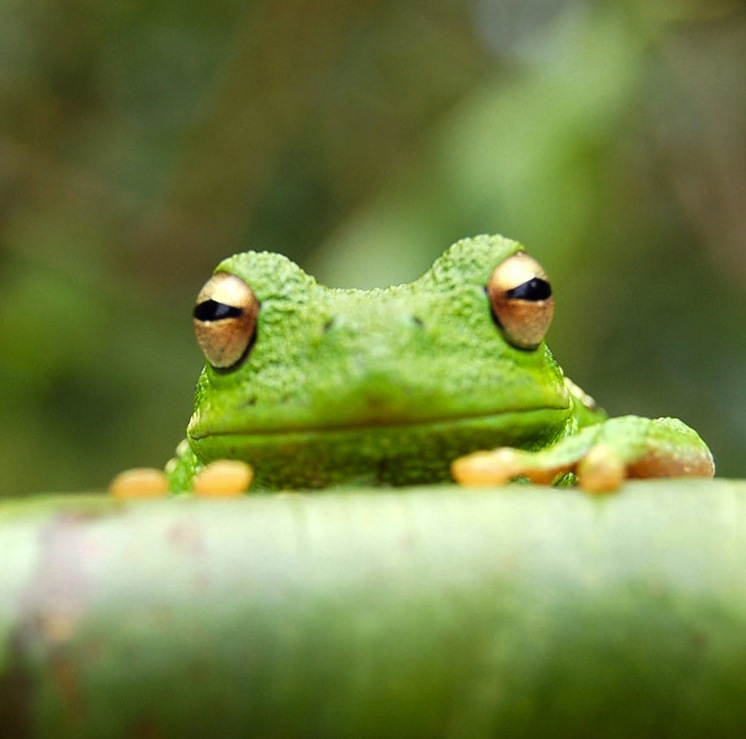
\includegraphics[width=0.3\textwidth]{frog.jpg}
% \caption{\label{fig:frog}This frog was uploaded via the project menu.}
% \end{figure}

% \subsection{How to add Tables}

% Use the table and tabular commands for basic tables --- see Table~\ref{tab:widgets}, for example. 

% \begin{table}
% \centering
% \begin{tabular}{l|r}
% Item & Quantity \\\hline
% Widgets & 42 \\
% Gadgets & 13
% \end{tabular}
% \caption{\label{tab:widgets}An example table.}
% \end{table}

% \subsection{How to write Mathematics}

% \LaTeX{} is great at typesetting mathematics. Let $X_1, X_2, \ldots, X_n$ be a sequence of independent and identically distributed random variables with $\text{E}[X_i] = \mu$ and $\text{Var}[X_i] = \sigma^2 < \infty$, and let
% \[S_n = \frac{X_1 + X_2 + \cdots + X_n}{n}
%       = \frac{1}{n}\sum_{i}^{n} X_i\]
% denote their mean. Then as $n$ approaches infinity, the random variables $\sqrt{n}(S_n - \mu)$ converge in distribution to a normal $\mathcal{N}(0, \sigma^2)$.


% \subsection{How to create Sections and Subsections}

% Use section and subsections to organize your document. Simply use the section and subsection buttons in the toolbar to create them, and we'll handle all the formatting and numbering automatically.

% \subsection{How to add Lists}

% You can make lists with automatic numbering \dots

% \begin{enumerate}
% \item Like this,
% \item and like this.
% \end{enumerate}
% \dots or bullet points \dots
% \begin{itemize}
% \item Like this,
% \item and like this.
% \end{itemize}

% \subsection{How to add Citations and a References List}

% You can upload a \verb|.bib| file containing your BibTeX entries, created with JabRef; or import your \href{https://www.overleaf.com/blog/184}{Mendeley}, CiteULike or Zotero library as a \verb|.bib| file. You can then cite entries from it, like this: \cite{greenwade93}. Just remember to specify a bibliography style, as well as the filename of the \verb|.bib|.

% You can find a \href{https://www.overleaf.com/help/97-how-to-include-a-bibliography-using-bibtex}{video tutorial here} to learn more about BibTeX.

% We hope you find Overleaf useful, and please let us know if you have any feedback using the help menu above --- or use the contact form at \url{https://www.overleaf.com/contact}!

\bibliographystyle{mn2e}
\bibliography{references}

\end{document}